\apendice{Manual del desarrollador} 

\section{Estructura de directorios}

El proyecto se ha organizado en una estructura de carpetas diferenciadas. A continuación, se describe el contenido y propósito de cada directorio:

\begin{itemize}
    \item \textbf{Artículos}: contiene una recopilación de artículos científicos y documentación técnica utilizada para la elaboración del estado del arte y la justificación de decisiones técnicas a lo largo del TFG. Dentro de ella, además de diferentes técnicas y métodos, hay un subdirectorio llamado \texttt{TFGs Pulsioxímetro}, en el que se pueden encontrar diferentes trabajos o proyectos que han desarrollado soluciones similares y que han servido de ayuda para entender cómo se han abordado problemas parecidos y qué soluciones se han propuesto en otros contextos.

   \item \textbf{Código}: incluye todos los scripts, algoritmos y archivos fuente del proyecto. Está dividido en subcarpetas:
\begin{itemize}

    \item \textbf{adquisición:} Contiene los scripts de Python que hay que ejecutar en el promt de Anaconda para poder registrar los datos y guardarlos en local en formato .csv en la ruta que se indique.
    
    \item \textbf{comparación}: contiene scripts para comparar los diferentes filtros descritos en el apartado de conceptos teóricos. Además, realiza una representación gráfica para observar el efecto de cada filtro sobre una señal PPG de ejemplo.
    
    \item \textbf{diagramas de bloques}: incluye esquemas visuales que representan el funcionamiento de los algoritmos y la arquitectura general del sistema.

    \item \textbf{firmware}: contiene el código embebido \textbf{original} que se ejecuta en la PCB de la incubadora. 

    \item \textbf{funciones modificadas:} en este directorio se encuentran los archivos \texttt{get\_AFE44XX\_Data\_modificada.cpp}, para la recogida de datos y \texttt{SPO2\_modificado.cpp}, que implementa el algoritmo de estimación de constantes fisiológicas. 
    
    \item \textbf{procesamiento}: contiene notebooks y scripts de Python para el tratamiento, filtrado y análisis de las señales registradas. También se calculan aquí los parámetros fisiológicos. Está organizado en dos carpetas principales, una para cada parámetro estimado, y dentro de cada una de ellas hay subcarpetas con pruebas, incluyendo procedimientos descartados.

    \item \textbf{resultados}: recoge las gráficas y tablas generados a partir del análisis de los algoritmos implementados en Python.
\end{itemize}


    \item \textbf{Datos}: estructura donde se almacenan los datos recogidos durante las sesiones de prueba. Se organiza en:
    \begin{itemize}
        \item \textbf{Datos crudos}: señales originales sin procesar. Se dividen en los directorios \texttt{save\_log} y \texttt{save\_log2}, según la versión de la función de adquisición que se haya utilizado.
        \item \textbf{Datos\_limpios}: señales tras la limpieza inicial, con un recorte \textbf{personalizado} para cada registro, según lo que sobrara de cada señal.
        \item \textbf{Procesados}: datos limpios, pero habiendo recortado para todos los registros, los primeros y últimos 5 segundos.
    \end{itemize}

    \item \textbf{Demostración}: vídeo corto de una simulación funcional de la solución desarrollada (formato \texttt{.mp4}).

    \item \textbf{Documentación de referencia}: manuales técnicos de los componentes utilizados (AFE4490, sensor UA401-D, normas ISO aplicables, documentación del proyecto \textit{In$^3$ator}, etc.). La mayoría cedidos por la ONG Medicina Abierta al Mundo.

    \item \textbf{Documentación Overleaf}: este es el proyecto principal en Overleaf donde se redacta tanto la memoria del TFG como los anexos. Está organizado en las siguientes carpetas y archivos:

    \begin{itemize}
        \item \texttt{tex/}: contiene los archivos `.tex` que forman los distintos capítulos de la memoria (introducción, metodología, resultados, etc.). 
        \item \texttt{img/}: carpeta con las imágenes, figuras y diagramas utilizados a lo largo del documento.
        \item \texttt{memoria.tex}: archivo principal que compila toda la memoria del TFG importando los capítulos desde la carpeta \texttt{tex}.
        \item \texttt{anexos.tex}: archivo donde se redactan todos los anexos del trabajo, también de forma modular.
        \item \texttt{bibliografia.bib}: fichero BibTeX con las referencias bibliográficas utilizadas en la memoria principal.
        \item \texttt{bibliografiaAnexos.bib}: archivo separado con las referencias citadas únicamente en los anexos, para mantener la bibliografía organizada y evitar duplicidades.
    \end{itemize}


    \item \textbf{README.md}: archivo de texto que resume el propósito del trabajo y explica brevemente cómo utilizar el proyecto.

    
    
\end{itemize}

\section{Requisitos software y hardware para ejecutar el proyecto.}

Este anexo está pensado para cualquier persona que quiera seguir desarrollando o mejorando este proyecto en el futuro.
Aquí se recopila todo lo necesario para compilar el código, programar la placa y entender cómo funciona por dentro el sistema de pulsioximetría.

Originalmente, parte de esta información estaba incluida en el Anexo B, pero como ese anexo está más enfocado a un usuario final, he decidido mover aquí todo lo relacionado con el entorno de desarrollo (como el sistema operativo, las herramientas usadas, o los drivers).
Así se mantiene más clara la distinción entre lo que necesita saber un usuario del sistema y lo que necesita saber alguien que quiera modificar o ampliar el software.

Este proyecto se ha desarrollado para funcionar en dos entornos complementarios:

\begin{itemize}
  \item \textbf{Entorno embebido}: ejecución del firmware en la placa electrónica de la incubadora neonatal \textit{In$^3$ator}, incluyendo la lectura de señales del sensor óptico y envío por puerto serie para obtener y estudiar los datos.
  \item \textbf{Entorno software}: ejecución en un ordenador de los scripts de adquisición, notebooks de procesamiento para obtener e interpretar los datos fisiológicos y firmware que imprime por el display los parámetros objetivo.
\end{itemize}

A continuación, se detallan los requisitos necesarios en ambos casos.

\subsection{Sistema operativo compatible}

\begin{itemize}
  \item \textbf{Windows 10/11}: entorno utilizado durante el desarrollo, compatible con todos los drivers y herramientas utilizadas.
  \item \textbf{Linux (Ubuntu 20.04+)}: compatible con modificaciones en permisos del puerto serie, aunque no fue el entorno de prueba principal.
\end{itemize}

El sistema también es compatible con \textbf{macOS}, aunque pueden ser necesarias configuraciones adicionales en los permisos del puerto serie y la instalación de drivers específicos para el programador EPS-Prog.

\subsection{Requisitos mínimos del ordenador}

Para garantizar un buen funcionamiento en la ejecución de los notebooks y del firmware con la interfaz de PlatformIO, se recomienda:

\begin{itemize}
  \item \textbf{Procesador}: Intel Core i5 o equivalente.
  \item \textbf{Memoria RAM}: al menos 8 GB. 
  \item \textbf{Espacio en disco}: mínimo 1 GB libre, recomendado 5 GB, para instalación de entornos virtuales, dependencias, notebooks y almacenamiento de logs en formato CSV.
  \item \textbf{Puertos}: al menos un puerto USB tipo A disponible para la conexión directa de la placa PCB a través del programador EPS-Prog (recomendable disponer de más de un puerto USB por si la conexión fallara).
\end{itemize}


\subsection{Software necesario}

\begin{itemize}
  \item \textbf{Anaconda}: el principal requisito de software para ejecutar este proyecto es tener instalado Anaconda Navigator. Ya que se ha utilizado Jupyter Notebook para el estudio previo de los datos y algoritmos.
  \item \textbf{Python}: lenguaje empleado para todos los scripts y notebooks de procesamiento.
  \item \textbf{Visual Studio Code (VSCode)}: entorno de desarrollo utilizado para desplegar y ejecutar el firmware.
  \item \textbf{Extensión PlatformIO para VSCode}: permite compilar, cargar y monitorizar el firmware en el microcontrolador.
  \item \textbf{Drivers FTDI para EPS-Prog}: necesarios para que el programador sea reconocido correctamente por el sistema operativo\footnotemark[1].
\end{itemize}

\footnotetext[1]{Para instalar el programador ESP-Prog, se siguieron las instrucciones oficiales de  \href{https://docs.platformio.org/en/stable/plus/debug-tools/esp-prog.html}{PlatformIO}}


\textbf{Versiones de cada elemento software}

\begin{table}[H]
  \centering
  \begin{tabular}{|l|l|}
    \hline
    \textbf{Elemento} & \textbf{Versión} \\
    \hline
    Python & 3.8.5 \\
    Anaconda & 4.9.2 \\
    Visual Studio Code & 1.99.3 (user setup) \\
    PlatformIO Core & 6.1.18 \\
    PlatformIO Home & 3.4.4 \\
    Driver FTDI & 2.12.36.4 \\
    \hline
  \end{tabular}
  \caption{Versiones exactas del entorno de desarrollo utilizado}
  \label{tab:versiones_software}
\end{table}

\section{Compilación, instalación y ejecución del proyecto}

Con el objetivo de que otra persona continúe con el desarrollo del proyecto, en esta sección se explica cómo hacer funcionar los distintos elementos del sistema desarrollado, tanto a nivel software como hardware.

Aunque durante la fase de implementación se optó por un enfoque basado en la adquisición de archivos \texttt{.csv} para analizar las señales y validar algoritmos antes de integrarlos en el firmware, este método ha sido una decisión personal para facilitar el desarrollo. Por tanto, en esta sección no se describe ese flujo específico de trabajo, sino simplemente la puesta en marcha general del sistema, tal como se necesitaría para hacerlo funcionar desde cero.


\subsection{Instalación del entorno software}

\begin{enumerate}
  \item \textbf{Instalación de Visual Studio Code (VSCode):}
  \begin{itemize}
    \item Descargar desde la web oficial de \href{https://code.visualstudio.com/}{VSCode} (Windows, Linux y MacOS).
    \item Ejecutar el instalador y seguir los pasos por defecto.
  \end{itemize}

  \begin{figure}[H]
  \centering
  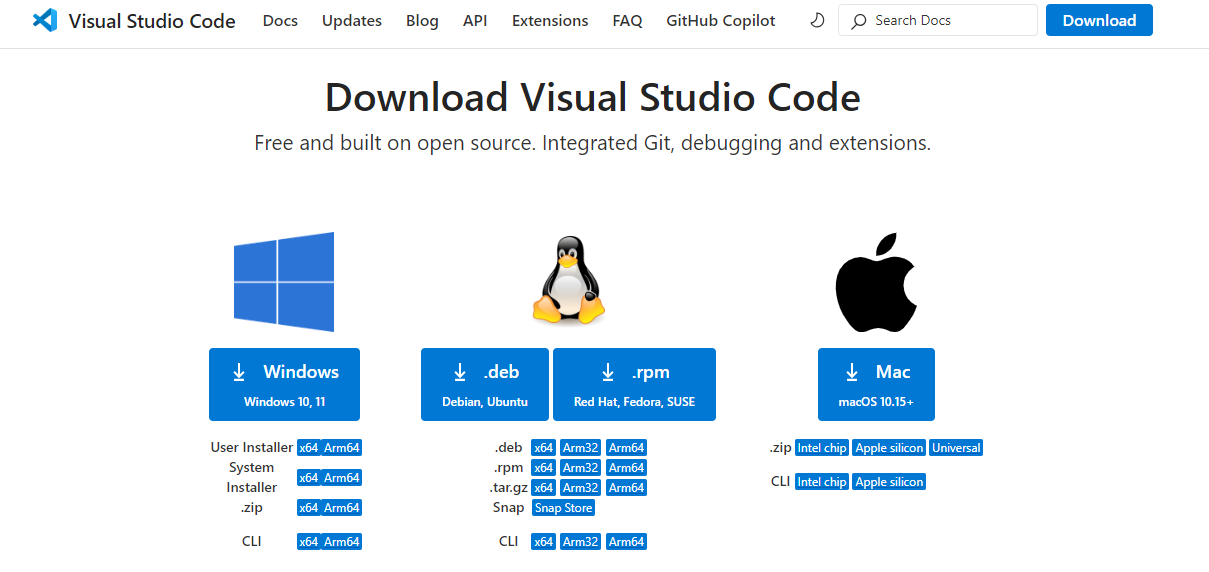
\includegraphics[scale =0.32]{img/vscode.png}
  \caption{Pantalla de instalación de Visual Studio Code. \textit{Elaboración propia.}}
  \label{fig:vscode_instalacion}
\end{figure}

  \item \textbf{Instalación de PlatformIO como extensión de VSCode:}
  \begin{itemize}
    \item Una vez abierto VSCode, hacer clic en el icono de extensiones (barra lateral izquierda).
    \item Buscar \texttt{PlatformIO IDE} y hacer clic en “Instalar”.
    \item Reiniciar VSCode tras la instalación para que la extensión se configure correctamente.
  \end{itemize}

  \begin{figure}[H]
  \centering
  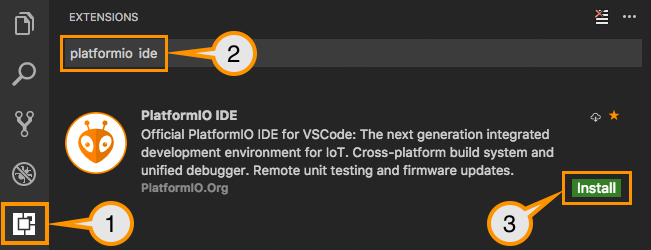
\includegraphics[width=0.65\textwidth]{img/platformio.png}
  \caption{Instalación de PlatformIO IDE desde el marketplace de Visual Studio Code. Fuente: \href{https://platformio.org/install/ide}{PlatformIO.}}
  \label{fig:platformio_instalacion}
\end{figure}

  \item \textbf{Instalación de Anaconda (incluye Python):}
  \begin{itemize}
    \item Descargar el instalador desde la página web de \href{https://www.anaconda.com/products/distribution}{Anaconda}.
    \item Seleccionar la versión para Windows e instalar con las opciones recomendadas.
    \item Anaconda incluye una instalación de Python, por lo que no es necesario instalarlo por separado.
  \end{itemize}

  \begin{figure}[H]
  \centering
  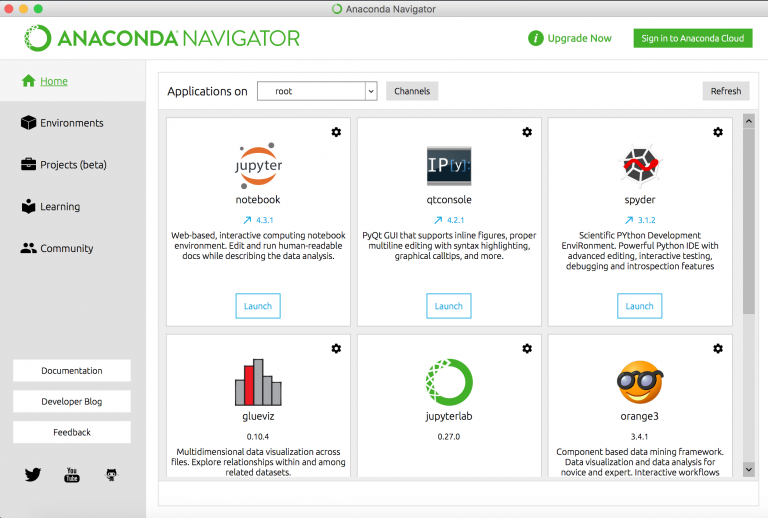
\includegraphics[width=0.65\textwidth]{img/anaconda-navigator.png}
  \caption{Instalación de Python desde Anaconda Navigator. Fuente: \href{https://www.aprendemachinelearning.com/instalar-ambiente-de-desarrollo-python-anaconda-para-aprendizaje-automatico/}{AprendeMachineLearning.}}
  \label{fig:anaconda_instalacion}
\end{figure}

  \item \textbf{Verificación de versiones de Python y Anaconda:}
  \begin{itemize}
    \item Abrir “Anaconda Prompt” y escribir:
    \begin{verbatim}
python --version
conda --version
    \end{verbatim}
    \item Deberían mostrarse las versiones instaladas. Las empleadas durante el desarrollo se recogen en la Tabla~\ref{tab:versiones_software}.
  \end{itemize}

  \item \textbf{Instalación de los drivers del programador EPS-Prog:}
  \begin{itemize}
    \item Es necesario instalar los drivers FTDI para que el programador sea reconocido como un puerto COM.
    \item Se puede seguir el tutorial oficial de \href{https://docs.platformio.org/en/stable/plus/debug-tools/esp-prog.html\#drivers}{PlatformIO.}
    \item Tras la instalación, el programador debe aparecer en el \textit{Administrador de dispositivos }de Windows bajo \textit{Puertos (COM y LPT)}.
    \item Para ello:
  \begin{itemize}
    \item Pulsar \texttt{Windows + R}, escribir \texttt{devmgmt.msc} y pulsar Enter o abrir directamente el \textit{Device Manager }desde el buscador de Windows.
    \item Desplegar el apartado \texttt{Puertos (COM y LPT)}.
    \item Debería aparecer una línea similar a \texttt{USB Serial Port (COM9)}.
  \end{itemize}
  \item Ese número de puerto (por ejemplo, \texttt{COM9}) será necesario para cargar el firmware, y en el caso de seguir esa metodología, para capturar datos con el script Python.
  \end{itemize}
\end{enumerate}

\subsection{Clonado y despliegue del firmware}

El código fuente original del firmware se encuentra disponible en el repositorio Git de la ONG, estructurado como un proyecto de PlatformIO. A continuación, se indican los pasos seguidos para clonar el proyecto, abrirlo en Visual Studio Code y cargarlo en la placa:

\begin{enumerate}
  \item \textbf{Clonado del repositorio:}
  \begin{itemize}
    \item Desde Visual Studio Code, abrir una nueva terminal.
    \item Ejecutar el comando:
    \begin{verbatim}
git clone https://github.com/medicalopenworld/in3ator.git
    \end{verbatim}
    \item También puede descargarse manualmente como archivo .zip y descomprimirse localmente\footnote{Dentro del repositorio, hacer click en el botón verde \texttt{Code} y seleccionar \texttt{Download ZIP}.}.
  \end{itemize}

  \item \textbf{Abrir el proyecto en PlatformIO:}
  \begin{itemize}
    \item Abrir VSCode y seleccionar la carpeta \texttt{Firmware/motherBoard}.
    \item PlatformIO detectará automáticamente el archivo \texttt{platformio.ini}, que define la configuración del proyecto.
    \item Verificar que la placa seleccionada sea la correcta (por ejemplo, ESP32) en dicho archivo.
  \end{itemize}

  \item \textbf{Compilación y carga del firmware:}
  \begin{itemize}
    \item Conectar la placa al ordenador mediante el programador EPS-Prog.
    \item Asegurarse de que el puerto COM detectado es el correcto.
    \item Desde la interfaz de PlatformIO (barra lateral izquierda), hacer clic en:
    \begin{itemize}
      \item \textbf{Build} (compilar el proyecto).
      \item \textbf{Upload} (cargar en el microcontrolador).
    \end{itemize}
    \item También puede hacerse desde terminal con:
    \begin{verbatim}
pio run --target upload
    \end{verbatim}
    \item Una vez cargado el firmware, se puede abrir el monitor serie desde PlatformIO (botón \textit{Monitor}) para verificar que la placa está enviando datos correctamente \footnote{Aunque el sensor no detecte el dedo, si el ordenador reconoce bien la placa, imprime los datos de las señales igualmente por la terminal.}.
  \end{itemize}
\end{enumerate} 

\subsection{Conexión del sistema físico}

Una vez instalado el entorno software y desplegado el firmware, el siguiente paso consiste en realizar las conexiones necesarias sobre la placa para que el sistema pueda funcionar correctamente y luego cargar el código que lee los datos. 

\textbf{Conectar la fuente de alimentación:}
  \begin{itemize}
    \item Utilizar una fuente de 12V con conector compatible.
    \item Conectarla a la entrada de alimentación de la PCB para suministrar energía al sistema.
  \end{itemize}

\textbf{Conectar el programador EPS-Prog:}
  \begin{itemize}
    \item Conectar el programador a la placa a través del cable JTAG a los pines correspondientes.
    \item Con un cable micro-USB, conectar el extremos micro-USB al programador y el extremo USB al ordenador. Una vez conectado, debería aparecer un nuevo puerto COM en el sistema.
  \end{itemize}

\textbf{Conectar el sensor óptico U401-D:}
  \begin{itemize}
    \item Conectar el sensor al conector designado en la placa.
    \item Asegurarse de que la orientación del conector sea correcta y que quede bien insertado.
  \end{itemize}


\section{Pruebas del sistema}
Para verificar el correcto funcionamiento del sistema completo, este apartado recoge las principales comprobaciones realizadas durante el desarrollo del sistema, para detectar posibles fallos en caso de que futuras personas retomen el proyecto y el sistema no funcione como se espera. 

Si tras seguir todos los pasos de instalación y despliegue, el sistema no responde correctamente, se recomienda revisar estos puntos para identificar en qué parte del proceso puede estar fallando.


\subsection{Comprobación del sensor óptico y alimentación de la placa}

Antes de acceder a los datos, lo primero que se debe comprobar es que el sensor óptico U401-D está correctamente conectado a la PCB y recibe alimentación. Al conectar la fuente de 12V, los LEDs del sensor deberían encenderse de forma visible. Si no se encienden aún estando conectado a la corriente eléctrica, pulsar el botón azul que se encuentra al reverso de la PCB.
\begin{figure}[H]
    \centering
    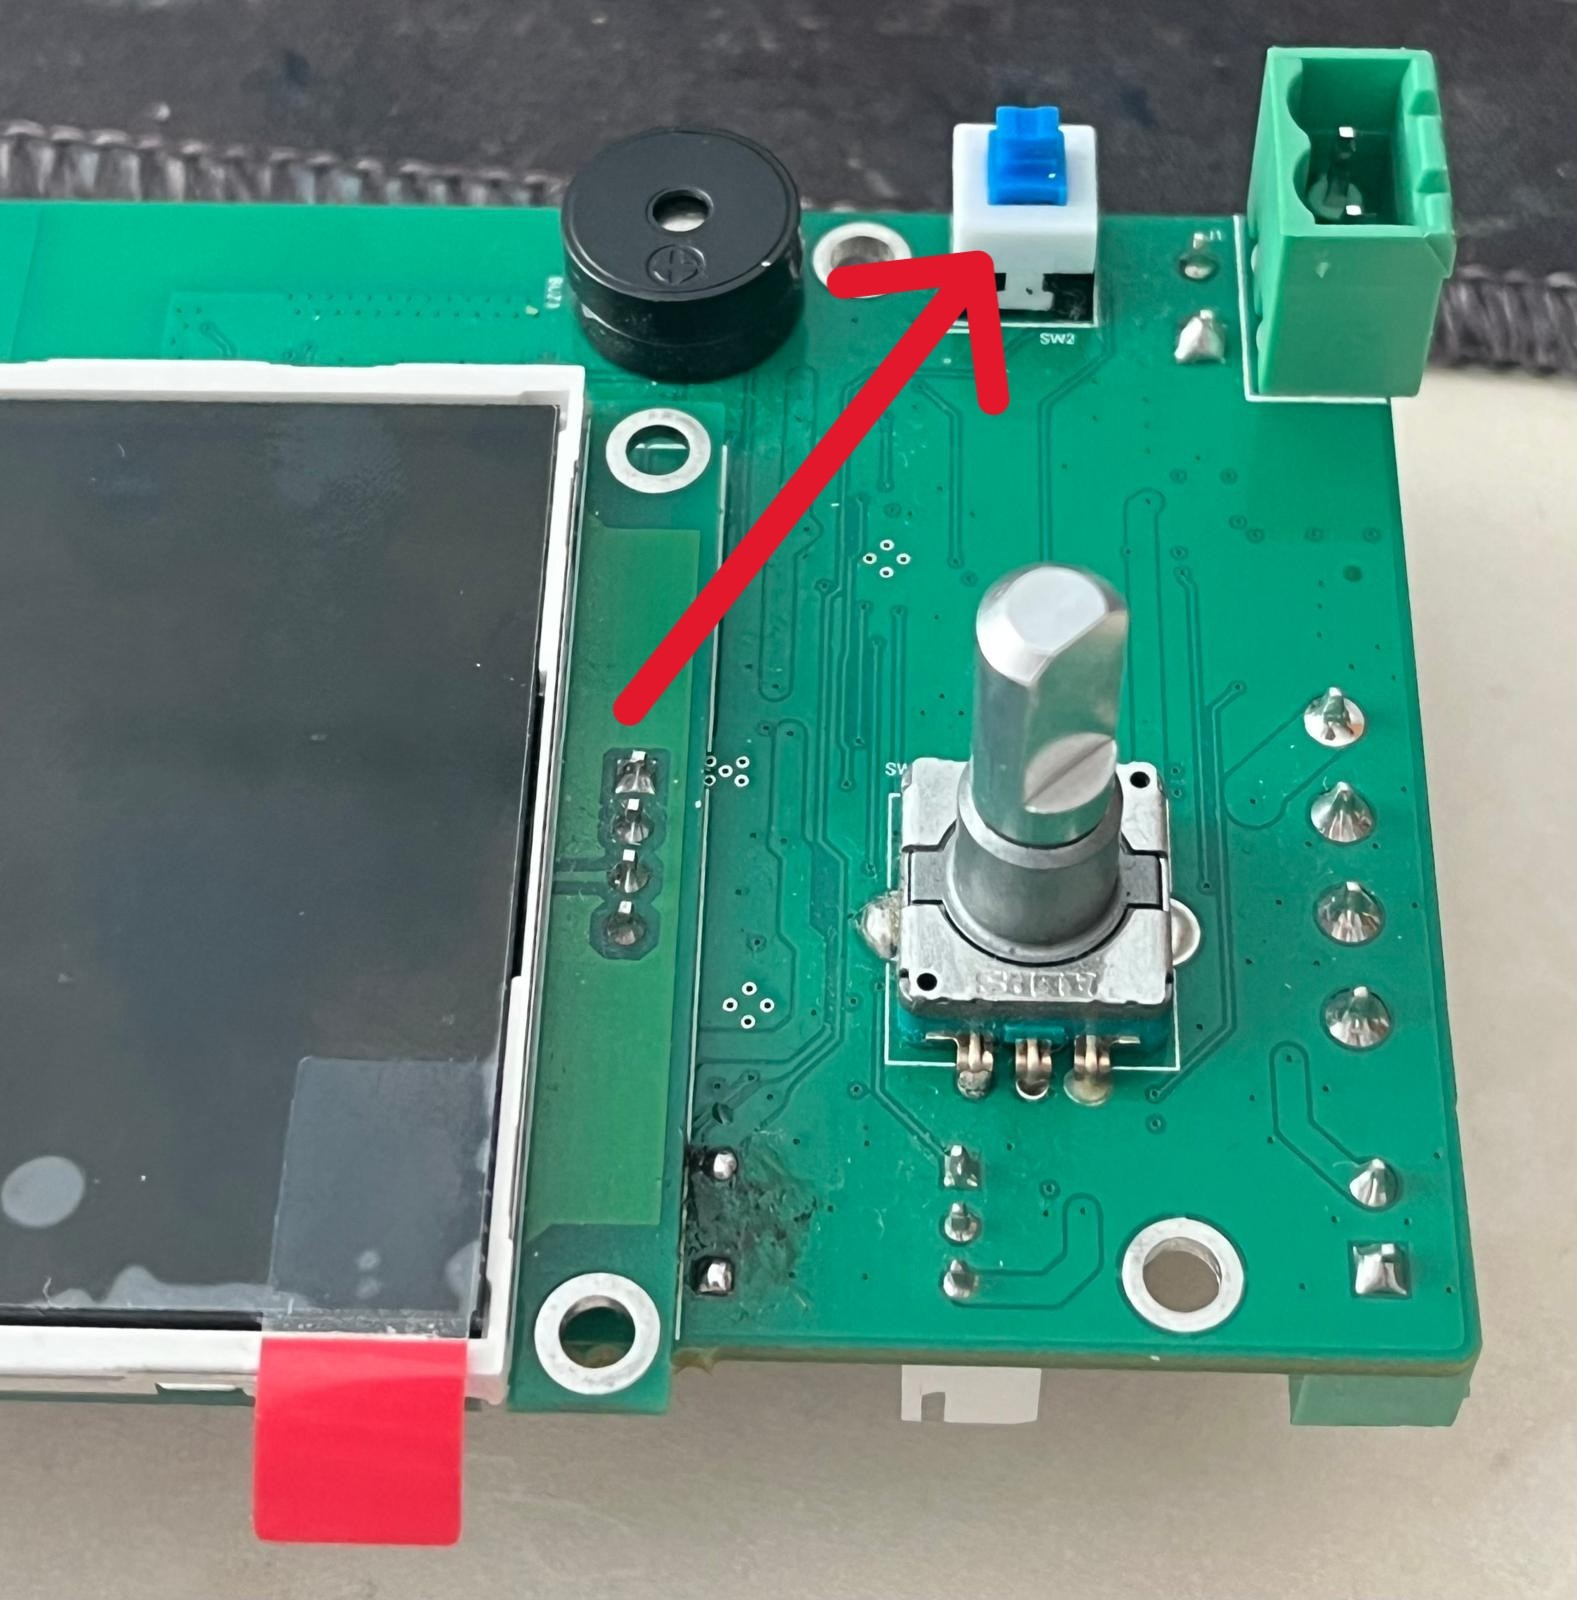
\includegraphics[width=0.5\linewidth]{img/boton.jpeg}
    \caption{Botón que enciende la placa si está apagada. \textit{Elaboración propia.}}
    \label{fig:botón}
\end{figure}
    
También es recomendable revisar que el conector esté orientado correctamente y bien insertado.

\subsection{Verificación de la comunicación por puerto serie}

Una vez asegurado que la placa está alimentada y que el sensor funciona, el siguiente paso es confirmar que el microcontrolador está enviando datos al ordenador a través del puerto serie. Esto puede comprobarse abriendo el monitor serie desde PlatformIO. 

Si el sistema está funcionando correctamente, al pulsar la opción \textit{Monitor} de PlatformIO deberían recibirse líneas con los valores crudos de los cuatro canales: IR, AMB\_IR, RED y AMB\_RED. Si no se recibe nada o aparecen símbolos extraños, puede ser que el puerto esté mal seleccionado o que el cable JTAG esté mal colocado.

Un aspecto importante a tener en cuenta es que el conector del programador puede colocarse de dos formas distintas, pero sólo es capaz de leer los datos en una de las posiciones. A continuación, se muestra la orientación correcta del cable plano sobre los pines de la placa. Es importante asegurarse de que la banda roja del cable queda alineada tal como se observa en la imagen \ref{fig: pines_prog}.

    \begin{figure}[H]
    \centering
    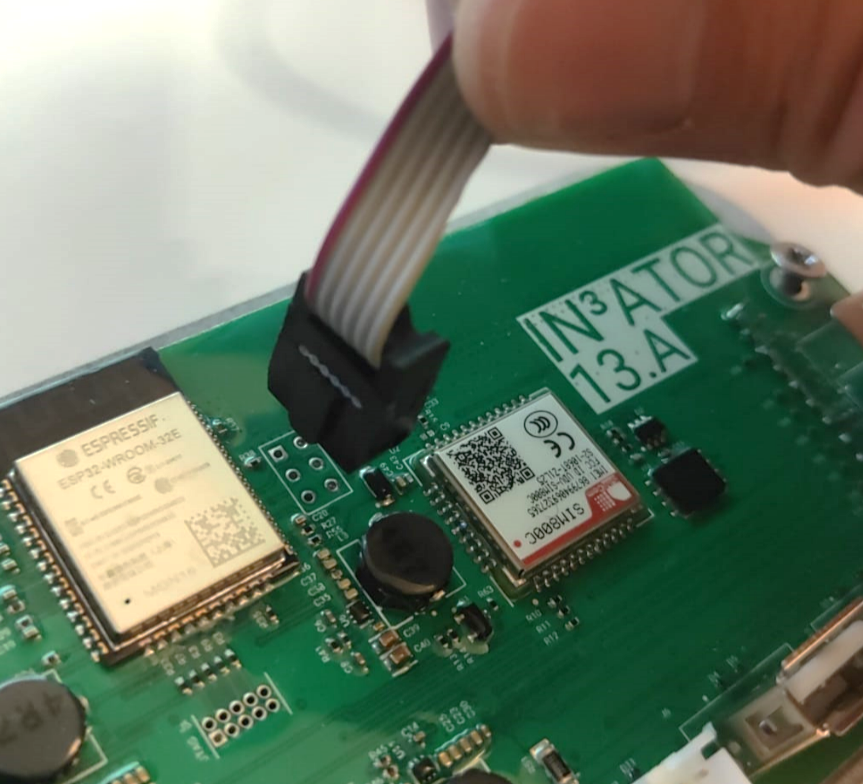
\includegraphics[width=0.5\textwidth]{img/pines_prog.png}
    \caption{Colocación correcta del cable del programador en la placa. \textit{Elaboración propia.}}
    \label{fig: pines_prog}
    \end{figure}

También es útil revisar en el Administrador de dispositivos (Windows) para ver si el programador EPS-Prog ha sido detectado como puerto COM. Si no aparece, el problema puede estar en los drivers FTDI o en la conexión física del programador.

\begin{figure}[H]
  \centering
  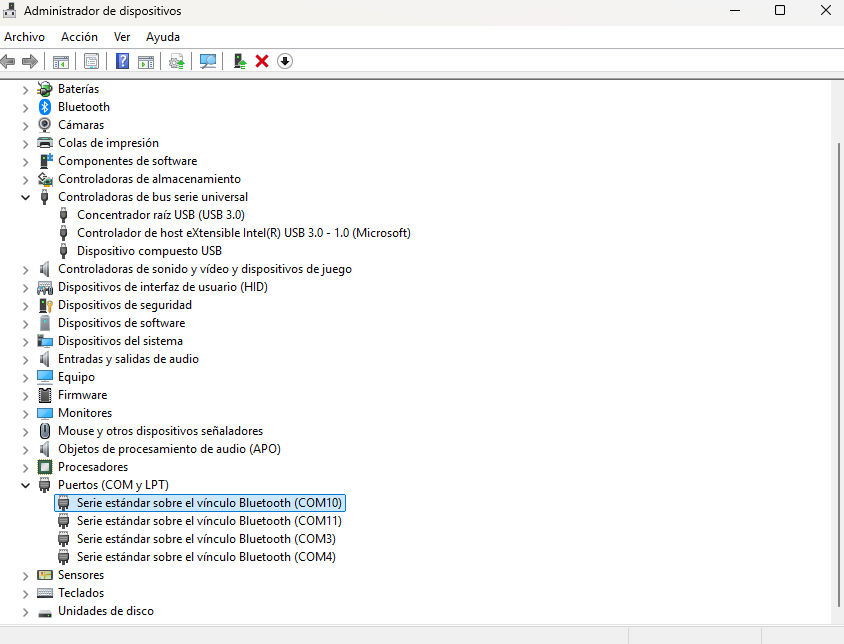
\includegraphics[width=0.85\textwidth]{img/device_manager.png}
  \caption{Interfaz del Device Manager de Windows \textbf{sin} el programador conectado.}
  \label{fig:device_manager}
\end{figure}

\begin{figure}[H]
  \centering
  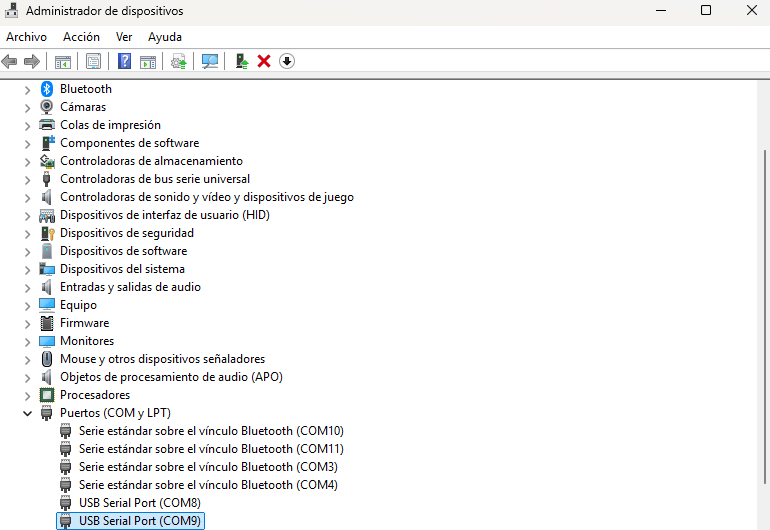
\includegraphics[width=0.85\textwidth]{img/device_manager2.png}
  \caption{Interfaz del Device Manager de Windows \textbf{con} el programador conectado.}
  \label{fig:device_manager2}
\end{figure}


\subsection{Alternativa de trabajo basada en archivos CSV}

En el caso de que se quieran validar los algoritmos directamente sobre el microcontrolador, se pueden recopilar en archivos .csv para analizarlos en Jupyter Notebook. Para seguir este enfoque y continuar haciendo pruebas adicionales a las presentadas, se recomienda utilizar el siguiente procedimiento:

Desde el firmware \textbf{original} del proyecto, intercambiar la función denominada \texttt{get\_AFE44XX\_Data}\footnote{Esta función modificada se encuentra dentro del directorio \texttt{Código.}} por la función modificada disponible en el repositorio de este TFG \footnote{\href{https://github.com/ElenaRuizMoreno/TFG-Elena-Ruiz/}{TFG-ElenaRuiz}}. Cargar el código en VSCode (mediante \textit{Upload} de PlatformIO) con los cambios realizados. Si se ha subido correctamente, tiene que aparecer lo siguiente:

\begin{figure}[H]
    \centering
    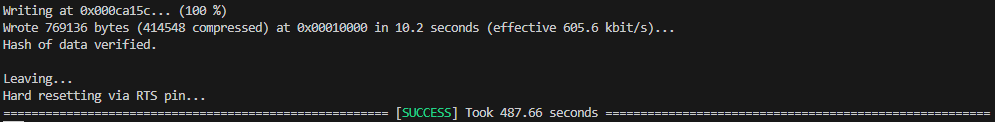
\includegraphics[scale=0.5]{img/succes.png}
    \caption{Mensaje que aparece al haber cargado el firmware correctamente en la PCB.}
    \label{fig:success}
\end{figure}


Descargar del repositorio el script \texttt{save\_log2.py}\footnote{El archivo se encuentra en el directorio \textit{procesamiento}, dentro del directorio principal \textit{Código}}. Este código lo que hace es leer datos desde la PCB conectada por puerto serie y guardarlos en un archivo CSV con una duración de 30 segundos y con las cabeceras correspondientes de cada columna. Para ello, hay que configurar tres cosas:

\begin{itemize}
    \item \texttt{SERIAL\_PORT = ``COMX"}: Define el puerto serie donde está conectada la PCB (comprobar a través del \textit{Device Manager} o PlatformIO)
    \item \texttt{BAUD\_RATE = 115200}: Establece la velocidad de transmisión de datos (115200 baudios), que debe coincidir con la del firmware de la placa\footnote{Este valor se puede encontrar dentro del archivo \texttt{platformio.ini} del proyecto, correspondiente a la variable \texttt{monitor\_speed}}.
    \item \texttt{OUTPUT\_FILE}: Especifica la ruta y nombre del archivo donde se guardarán los datos CSV. Cambiar según donde se quiera almacenar.
\end{itemize}

Una vez configuradas estas especificaciones, ejecutar el fichero en el Prompt de \textit{Anaconda} con el comando \texttt{python save\_log2.py} en la ruta del directorio donde esté ubicado. A la vez que se ejecuta, el sensor debe estar colocado en el dedo evitando exceso de luz o movimiento durante los segundos que dura cada registro. 

Es importante comprobar que los archivos generados contienen las columnas esperadas y que los valores cambian con el tiempo (es decir, que no son todos ceros o constantes). Si el archivo está vacío o con líneas incompletas, puede deberse a errores de lectura, desconexiones intermitentes o saturación del buffer serie.

\section{Instrucciones para la modificación o mejora del proyecto.}

Con el fin de ampliar o adaptar el sistema actual, a continuación, se describen los elementos del código y del hardware que se deben tener en cuenta para realizar cambios o implementar mejoras.

En cuanto al hardware y sus conexiones físicas, es importante tener en cuenta que el sistema ha sido desarrollado utilizando el material facilitado por la ONG Medicina Abierta al Mundo. Los componentes mencionados son los que se prevé utilizar en caso de que el proyecto se consolide y pase a emplearse de forma real en las incubadoras. Por tanto, no se recomienda modificar ni sustituir estos elementos, ni alterar su forma de conexión, ya que el diseño actual responde a limitaciones de coste y criterios de disponibilidad y compatibilidad definidos por la organización. 

\subsection{Modificación de algoritmos de procesamiento}

Los algoritmos de estimación de frecuencia cardíaca y SpO$_2$ se encuentran implementados inicialmente en formato notebook (\texttt{procesamiento/}) para su validación sobre datos en CSV. En caso de querer incluir nuevos algoritmos y estimaciones para después llevarlo al firmware, se recomienda:

\begin{itemize}
    \item Validar el nuevo algoritmo primero en Jupyter Notebook.
    \item Extraer las funciones clave y convertirlas a C++.
    \item Sustituir las funciones dentro de las funciones \texttt{spo2\_algorithm.cpp} y/o \texttt{hr\_estimation.cpp} según corresponda.
\end{itemize}

\subsection{Ajuste de parámetros de adquisición}

En el archivo \texttt{platformio.ini}, es posible modificar:

\begin{itemize}
    \item \texttt{monitor\_speed}: velocidad de transmisión por puerto serie.
    \item \texttt{build\_flags}: definición de macros para configurar el comportamiento del firmware.
\end{itemize}

Dentro del código fuente, pueden ajustarse:

\begin{itemize}
    \item Tiempo de adquisición por registro.
    \item Frecuencia de muestreo.
    \item Umbrales de detección de picos.
\end{itemize}

\subsection{Ampliación de funcionalidades}

Algunas ideas de ampliación que pueden llevarse a cabo directamente sobre la base del código existente:

\begin{itemize}
    \item Añadir visualización gráfica de la señal en la pantalla TFT (requiere librerías gráficas).
    \item Guardar registros en una tarjeta SD o memoria interna.
    \item Implementar conexión Bluetooth para enviar los datos a una app externa.
\end{itemize}